% One agent, one round, in the 8-agent population (myth-then-game order).
% Grounded in src/simulation.py (task loop), src/myth_writer.py
% (get_myth_prompt_round_later: shown myth = previous round's partner's myth),
% games/trust_game_noisy.py (_format_multi_agent_history, _finalize_game_prompt),
% src/agents.py (_truncate_messages: memory_capacity 6 pairs = 3 rounds),
% config/experiments_noisy.yaml: noisy8_crossmodel_negative_twotask_r3.
\documentclass[tikz,border=8pt]{standalone}
\usepackage[T1]{fontenc}
\usepackage{lmodern}
\renewcommand{\familydefault}{\sfdefault}
\usetikzlibrary{arrows.meta,positioning,calc}
\begin{document}
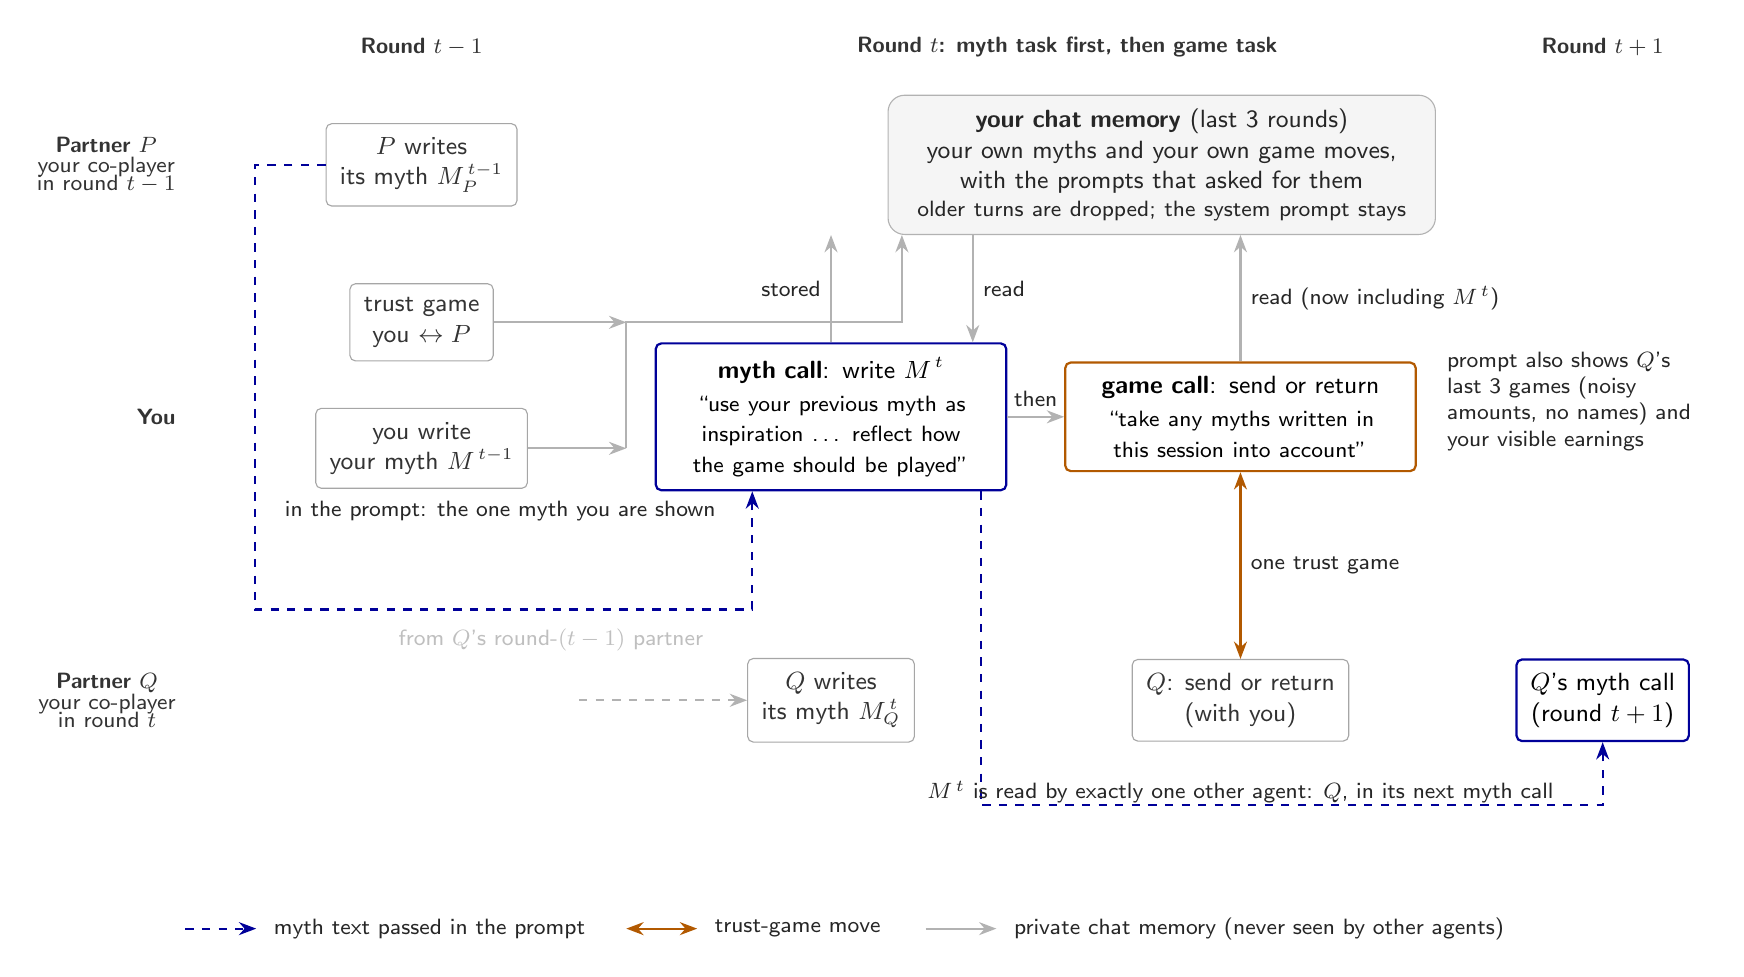
\begin{tikzpicture}[
  font=\small,
  >={Stealth[length=2.2mm]},
  call/.style={draw, rounded corners=2pt, fill=white, align=center, inner sep=5pt, minimum height=9mm},
  mythcall/.style={call, draw=blue!60!black, thick, text width=4.1cm},
  gamecall/.style={call, draw=orange!70!black, thick, text width=4.1cm},
  other/.style={call, draw=gray!70, text=gray!40!black},
  memory/.style={draw=gray!60, fill=gray!8, rounded corners=6pt, align=center, inner sep=5pt, text=gray!30!black},
  mythflow/.style={->, thick, blue!60!black, dashed},
  gameflow/.style={<->, thick, orange!70!black},
  memflow/.style={->, gray!60, thick},
  note/.style={font=\footnotesize, align=center, text=gray!30!black},
  lab/.style={font=\footnotesize\bfseries, text=gray!40!black, align=center},
]
% ---- column headers and row labels
\node[lab] at (0,4.7)    {Round $t-1$};
\node[lab] at (8.2,4.7)  {Round $t$: myth task first, then game task};
\node[lab] at (15.0,4.7) {Round $t+1$};
\node[lab, anchor=east] at (-3.0,3.2)  {Partner $P$\\[-2pt]\footnotesize\mdseries your co-player\\[-3pt]\footnotesize\mdseries in round $t-1$};
\node[lab, anchor=east] at (-3.0,0)    {You};
\node[lab, anchor=east] at (-3.0,-3.6) {Partner $Q$\\[-2pt]\footnotesize\mdseries your co-player\\[-3pt]\footnotesize\mdseries in round $t$};

% ---- round t-1
\node[other] (Pmyth)  at (0,3.2)  {$P$ writes\\its myth $M_P^{\,t-1}$};
\node[other] (Pgame)  at (0,1.2)  {trust game\\you $\leftrightarrow P$};
\node[other] (Ymyth0) at (0,-0.4) {you write\\your myth $M^{\,t-1}$};

% ---- round t: you
\node[mythcall] (Ymyth) at (5.2,0) {\textbf{myth call}: write $M^{\,t}$\\[1pt]\footnotesize``use your previous myth as inspiration \ldots\ reflect how the game should be played''};
\node[gamecall] (Ygame) at (10.4,0) {\textbf{game call}: send or return\\[1pt]\footnotesize``take any myths written in this session into account''};
\node[memory, text width=6.6cm] (mem) at (9.4,3.2) {\textbf{your chat memory} (last 3 rounds)\\your own myths and your own game moves, with the prompts that asked for them\\[-1pt]\footnotesize older turns are dropped; the system prompt stays};

% ---- round t: Q
\node[other] (Qmyth) at (5.2,-3.6)  {$Q$ writes\\its myth $M_Q^{\,t}$};
\node[other] (Qgame) at (10.4,-3.6) {$Q$: send or return\\(with you)};

% ---- round t+1
\node[call, draw=blue!60!black, thick] (Qnext) at (15.0,-3.6) {$Q$'s myth call\\(round $t+1$)};

% ---- the one myth you are shown (P's), routed around the left
\draw[mythflow] (Pmyth.west) -- ++(-0.9,0) |- ($(Ymyth.south)+(-1.0,-1.5)$) -- ($(Ymyth.south)+(-1.0,0)$)
;
\node[note, anchor=south] at (1.0,-1.45) {in the prompt: the one myth you are shown};

% ---- memory: round t-1 events go in
\draw[memflow] (Pgame.east)  -- (2.6,1.2);
\draw[memflow] (Ymyth0.east) -- (2.6,-0.4);
\draw[memflow] (2.6,-0.4) -- (2.6,1.2) -| ($(mem.south)+(-3.3,0)$);
% ---- memory and the two calls
\coordinate (st) at ($(Ymyth.north)+(0.0,0)$);
\coordinate (rd) at ($(mem.south)+(-2.4,0)$);
\draw[memflow] (st) -- node[note, left]{stored} (st |- mem.south);
\draw[memflow] (rd) -- node[note, right]{read} (rd |- Ymyth.north);
\draw[memflow] (Ygame.north) -- node[note, right]{read (now including $M^{\,t}$)} (Ygame.north |- mem.south);
\draw[memflow] (Ymyth.east) -- node[note, above]{then} (Ygame.west);

% ---- the game
\draw[gameflow] (Ygame.south) -- node[note, right]{one trust game} (Qgame.north);
\node[note, anchor=north west, text width=3.3cm, align=left] at (12.9,0.95) {prompt also shows $Q$'s last 3 games (noisy amounts, no names) and your visible earnings};

% ---- where your myth goes
\draw[mythflow] ($(Ymyth.south)+(1.9,0)$) |- ($(Qnext.south)+(0,-0.8)$) -- (Qnext.south)
;
\node[note, anchor=north] at (10.4,-4.5) {$M^{\,t}$ is read by exactly one other agent: $Q$, in its next myth call};
% Q does the same
\draw[mythflow, gray!60] (2.0,-3.6) -- (Qmyth.west);
\node[note, anchor=south east, text=gray!50] at (3.7,-3.1) {from $Q$'s round-$(t-1)$ partner};

% ---- legend
\begin{scope}[shift={(-3.0,-6.5)}]
  \draw[mythflow] (0,0) -- (0.9,0); \node[note, anchor=west] at (1,0) {myth text passed in the prompt};
  \draw[gameflow] (5.6,0) -- (6.5,0); \node[note, anchor=west] at (6.6,0) {trust-game move};
  \draw[memflow] (9.4,0) -- (10.3,0); \node[note, anchor=west] at (10.4,0) {private chat memory (never seen by other agents)};
\end{scope}
\end{tikzpicture}
\end{document}
